% 12. Стадия 1b
\begin{frame}{Стадия 1b · Traffic-BERT}
\framesubtitle{Bi-Cross Attention для двух признаковых последовательностей}
\vspace{1mm}
\begin{columns}[T,onlytextwidth]
\column{0.44\textwidth}
  \centering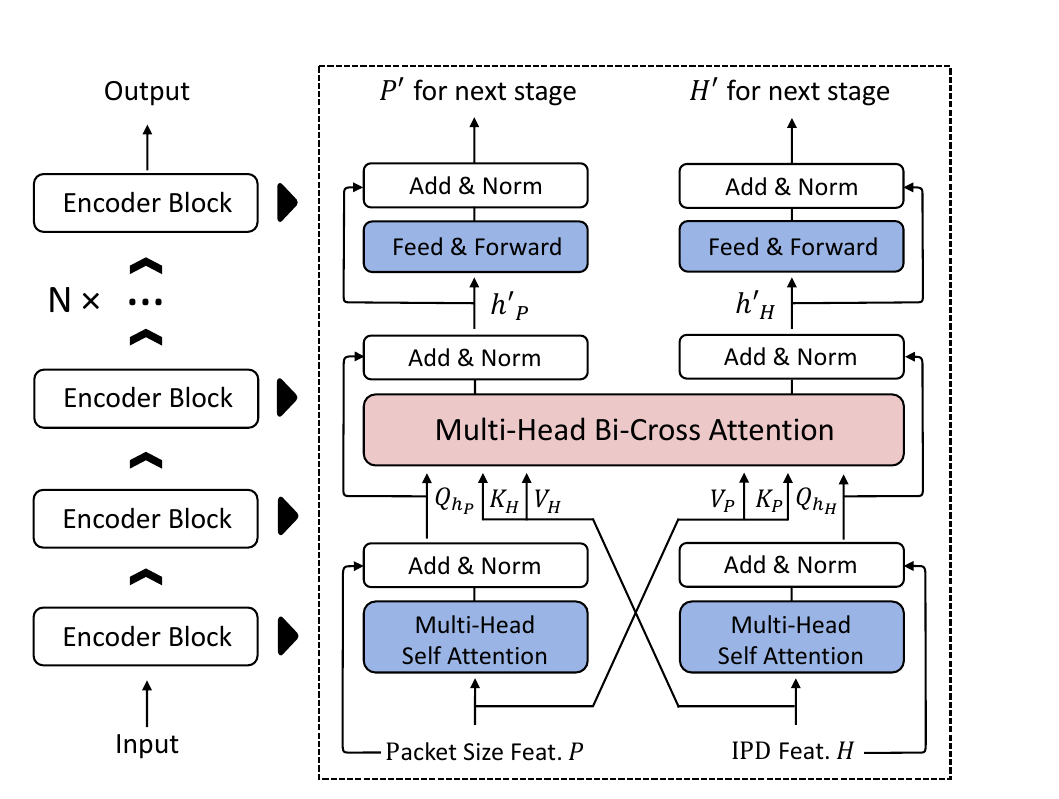
\includegraphics[width=\linewidth,height=5.9cm,keepaspectratio]{fig5.png}
\column{0.53\textwidth}
\begin{card}
  \cardtitle{Bi-Cross Attention}
  Каждый блок = self-attention (внутри последовательности) + двунаправленный cross-attention (размер $\leftrightarrow$ IPD) + FFN. Одна последовательность запрашивает другую и наоборот — та же сложность $O(n^2 d_k)$.
\end{card}\par\vspace{4mm}
\begin{darkcard}
  \iconitem{accent}{ic_flask_w.png}{\bfseries\small\color{accentlt}Задача Mask-Fill}\par\vspace{2mm}
  Маскируем 15\% позиций в обеих последовательностях сразу (80\% [MASK] / 10\% случайный / 10\% без изменений). Модель учится достраивать реалистичные benign-пакеты по контексту.
\end{darkcard}
\end{columns}
\end{frame}
